\chapter{Introducción}

El objetivo de este proyecto es evitar que un sistema \textit{blockchain} sea vulnerable a futuros ataques cuánticos. Para ello se ha implementado un algoritmo criptográfico resistente a ordenadores cuánticos, denominado \acrshort{uov}, para la firma de bloques, y posteriormente se ha integrado en la \textit{blockchain} ARK.

\section{Motivación y contexto del proyecto}
\label{sec:intro:motivacion} %Esto se pone si queremos hacer referencia a esta sección

%En esta parte es importante clarificar las siguientes preguntas: 
%\begin{enumerate}
%\item ¿Cuál es el problema que pretendemos resolver con este proyecto? Debemos introducir un poco el contexto en el que aparece y describir bien en qué consiste dicho problema. 
%\item ¿Por qué es importante dicho problema? Hay que tratar de aportar datos y argumentos para indicar que el problema descrito es relevante en el contexto actual. 
%\end{enumerate}

La tecnología ha transformado nuestra sociedad en una sociedad digitalizada, donde actualmente, los dispositivos digitales comportan la mayor parte de nuestras actividades diarias en distintos ámbitos, como económicas, organizativas o sociales. En el proceso de digitalización de la sociedad podemos distinguir las siguientes cinco fases \cite{fases-digitalizacion}.\\

La primera fase o era del Internet, corresponde a mediados de los 90. En esta fase se comenzaron a crear páginas web para que los medios de comunicación y las empresas puedieran publicar y compartir información.\\

La segunda fase o era de las redes sociales, tuvo mayor auge a partir de 2005. Plataformas de bajo o ningún coste, se utilizaban en las empresas para poder llegar mejor a los clientes.\\

La tercera fase o era de la economía colaborativa, nació con la crisis de  2008 cuando las empresas tenían pocos recursos. Surgieron plataformas para conectar a las personas, y poder obtener lo que necesitasen unas de otras. Por ejemplo pagos online, ver recomendaciones y reseñas de un alojamiento o pedir un taxi. Además se da un gran paso ya que estas aplicaciones pasan de estar  alojadas en ordenadores a teléfonos inteligentes.\\

La cuarta fase o era del mundo autónomo, se ha desarrollado durante décadas. Se desarrollan tecnología con inteligencia artificial, es decir, que simulan la inteligencia de los humanos para poder resolver problemas más complejos.\\

Quinta fase o era del bienestar moderno, comienza con las pulseras inteligentes como \textit{Fitbit} o \textit{Fuelband} de Nike. Estas pulseras son el impulso de la tecnología para facilitar la vida de los clientes y poder integrar la tecnología en la vida de los mismos.\\

La digitalización debe de venir acompañada de mecanismos que aporten seguridad a los datos. Los pilares de la seguridad de la información son los conocidos como la tríada CIA (confidencialidad, integridad y  disponibilidad)\cite{servicios-seguridad}.\\

La \textbf{confidencialidad} es la propiedad que impide que la información pueda ser accesible por entidades no autorizadas. Un sistema garantiza la confidencialidad cuando un tercero entra en posesión de la información intercambiada entre el remitente y el destinatario, no es capaz de extraer ningún contenido legible. Para asegurar la confidencialidad se utilizan mecanismos de cifrado y ocultación de la comunicación.\\

La \textbf{integridad} busca mantener la exactitud de los datos, es decir, que no hayan sido modificados durante su envío. La integridad se obtiene adjuntando al mensaje otro conjunto de datos de comprobación de la integridad, un ejemplo es la firma digital.\\

La \textbf{disponibilidad} es la cualidad de la información de encontrarse a disposición de quienes deben acceder a ella, ya sean personas, procesos o aplicaciones, en los momentos que así lo quieran. Los mecanismos para asegurar la disponibilidad se implementan con la infraestructura tecnológica.\\

Además de estos tres pilares hay otro principio, la \textbf{autentificación}, que es la propiedad que permite identificar al generador de la información. Trata de comprobar si un mensaje enviado por un usuario, ha sido verdaderamente firmado por él mismo. Esto se consigue con el uso de cuentas de usuario y contraseñas de acceso.\\

Para garantizar estos servicios de seguridad se hace uso de protocolos de seguridad de la información entre los que se encuentra la criptografía, la lógica y la autenticación.\\

La criptografía se ocupa de cifrar ciertos mensaje con el fin de hacerlos ilegibles a receptores no autorizados, una vez que llega a su destino y sea descifrado, el receptor obtendrá el mensaje original \cite{criptografia}. Además dota de seguridad a las comunicaciones, a la información y a las entidades que se comunican.\\

%\newpage
Podemos diferenciar dos tipos de criptografía, la criptografía simétrica y la asimétrica. La criptografía simétrica utiliza la misma clave para cifrar y descrifrar un mensaje, esta clave la ha de conocer tanto el emisor como el receptor. Mientras que la asimétrica utiliza dos claves la pública y la privada.\\

En la criptografía asimétrica podemos diferenciar dos ramas, el cifrado de clave pública y las firmas digitales \cite{criptografia-asimetrica}. En el cifrado de clave pública, el emisor cifra el mensaje con la clave pública del destinatario y el receptor lo descifra con su propia clave privada. En las firmas digitales, el emisor firma el mensaje con su clave privada y el receptor puede verificar el mensaje con su propia clave pública, además cualquier manipulación del mensaje se refleja en su resumen o \textit{hash}.\\

Este tipo de criptografía basa su seguridad en la hipótesis de que no se pueden encontrar las claves por fuerza bruta con la tecnología existente en la actualidad. Los ataque de fuerza bruta tratan de recuperar las claves probando todas las posibles combinaciones hasta encontrar la que permite el acceso, a partir del algoritmo de cifrado y del texto cifrado con su original \cite{fuerza-bruta}. Para que la búsqueda tenga éxito se deberán de realizar $10^n-1$ operaciones donde $n$ es la longitud de la clave.\\

Otro factor importante, en la seguridad, es si en la clave aparecen números, caracteres o la combinación de ambos, aumentando así el coste de encontrar las claves, llegando a alcanzar tiempos de cálculo logarítmicos, es decir, que podrían tardar siglos en encontrar una contraseña compleja pero también depende de la capacidad de operación del ordenador.\\

En este contexto, la aparición de la futura computación cuántica permitirá el cálculo de operaciones a una velocidad mucho mayor. En la figura \ref{fig:comp-clasica-cuantica} podemos observar la capacidad de cómputo del peor ordenador cuántico, con la línea continua, que sigue la gráfica de una función exponencial, frente a la capacidad del mejor ordenador clásico, la línea discontinua, que sigue una función lineal.\\

\begin{figure}[H]
	\centering
	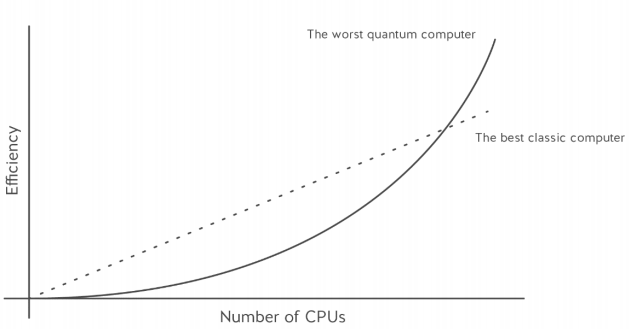
\includegraphics[width=0.55\textwidth]{figuras/comp_clasica_cuantica.png}
	\caption{Comparativa de la capacidad de cómputo de un ordenador clásico con un ordenador cuántico\cite{clasica-vs-cuantica}}
	\label{fig:comp-clasica-cuantica}
\end{figure}

La comparativa también nos muestra que para operaciones pequeñas como, por ejemplo, editar un documento de texto un ordenador cuántico sería probablemente ineficiente. Por tanto lo mejor sería un ordenador híbrido, que mezclase computación clásica, para cálculos pequeños, y computación cuántica, para operaciones de mayor tamaño.\\

Cuando esté desarrollado el ordenador cuántico no serán válidos los actuales algoritmos criptográficos de clave pública, como \acrshort{rsa}, Diffie-Hellman y \mbox{\acrshort{ecdsa}}, ya que se basan en los problemas del logaritmo discreto y factorización de enteros, resolubles fácilmente por un ordenador cuántico. Las primeras ideas de la criptografía cuántica aparecieron en los años 70, destacando los algoritmos de Shor y Grover.\\

Veamos la tabla comparativa \ref{table:security-level}. Esta nos indica el tipo de algoritmo criptográfico, el algoritmo con la longitud de la clave y a continuación el nivel de seguridad tanto en un ordenador clásico como en uno cuántico. El nivel de seguridad de un algoritmo nos indica el número de operaciones necesarias para romper dicho algoritmo, por ejemplo, si tiene un nivel de seguridad $n$ entonces se requieren $2^n$ operaciones para romper el algoritmo \cite{security-level}. Observamos que hay una diferencia considerable en los niveles de seguridad de los algoritmo asimétricos, puesto que con un ordenador clásico al menos se necesitan $2^{112}$ operaciones mientras que con computación cuántica solo una. \\

\begin{table}[H]
	
	
	\centering
	\resizebox{\linewidth}{!}{
	\begin{tabular}{c c c c c }
		\hline \\[-1.5ex]
		\thead{Tipo} & \thead{Algoritmo-Longitud clave} & \thead{Nivel seguridad\\ (ordenador clásico)} & \thead{Nivel seguridad\\ (ordenador cuántico)} & \thead{Ataque cuántico}\\ [1ex] 
		\hline\hline \\[-1.5ex]
		\multirow{4}{5em}{Asimétrico} & RSA-2048 & 112 & 0 & Algoritmo de Shor \\ [0.5ex]
		& RSA-3072 & 128 & 0 & Algoritmo de Shor \\ [0.5ex]
		& ECC-521 & 128 & 0 & Algoritmo de Shor \\ [0.5ex]
		& ECC-521 & 256 & 0 & Algoritmo de Shor \\ [0.5ex]
		\hline \\[-1.5ex]
		\multirow{2}{5em}{Simétrico} & AES-128 & 128 & 64 & Algoritmo de Grover \\ [0.5ex]
		& AES-256 & 256 & 128 & Algoritmo de Grover \\ [1ex]
		\hline
	\end{tabular}}
	\caption{Niveles de seguridad de ordenadores clásicos y cuánticos \cite{security-bit}}
	\label{table:security-level}
\end{table}


En la actualidad, se están desarrollando muchos algoritmos para que sean resistentes a ataques de tipo cuántico, denominados algoritmos de criptografía postcuántica \cite{criptografia-postcuantica}. Estos ataques afectan principalmente a los algoritmos de clave pública o asimétrica, puesto que para la criptografía simétrica duplicar el tamaño de clave empleada es suficiente para hacerlos seguros y hacer inservible el algoritmo de Grover.\\

\newpage
Por otro lado, también en la actualidad está siendo muy relevante la adopción de las \textit{blockchain} como tecnología para ofrecer diversos servicios. Las \textit{blockchain} o cadenas de bloques son listas de transacciones, denominadas bloques, firmadas y unidas con algoritmos criptográficos. Además cada bloque contiene el hash del bloque anterior, lo que se explicará con más detalle en la sección \ref{sec:intro:blockchain}.\\

Esta tecnología se ha integrado en diferentes áreas, donde resalta el uso en los servicios financieros o criptomonedas, que aumenta la eficiencia y disminuye los costes. Otro uso de las \textit{blockchain} es en las cadenas de suministro, algunos restaurantes, como Fogo de Ch\~{a}o \cite{Fogo-Chao}, están empezando a utilizar las \textit{blockchain} para poder rastrear el origen de sus alimentos hasta llegar al propio restaurante, una gran ventaja para encontrar fácilmente si hay algún producto contaminado o en mal estado. \\

Un ejemplo del uso de las \textit{blockchain} queda reflejado en este proyecto en el que se ha implementado un algoritmo resistente a ataques cuánticos, \acrshort{uov} \cite{algoritmo-UOV} y se ha adaptado a la \textit{blockchain} ARK \cite{ark} para que se utilice dicho algoritmo de firma.\\


\section{Objetivos del proyecto y logros conseguidos}
\label{sec:intro:objetivos}
El objetivo de este proyecto es modificar el algoritmo de firma y verificación de los bloques de la \textit{blockchain} ARK, para hacerla resistente a ataques cuánticos.\\

\begin{itemize}
	\item Implementación del algoritmo \acrshort{uov}: Se ha implementado las funciones de generación de claves tanto públicas como privadas, la función de firma a partir de la clave privada y la función de verificación de la misma con la clave pública. Además ha sido necesario implementar la aritmética de cuerpo finito de $2^7$ elementos.
	\item Integración del algoritmo \acrshort{uov} en la \textit{blockchain} ARK para comprobar su funcionamiento: Se ha modificado el algoritmo de firma dado en la \textit{blockchain} por el algoritmo \acrshort{uov} para aumentar la seguridad.

\end{itemize}


\section{Estructura de la memoria}
%Se describirán los capítulos que tiene la memoria, indicando qué contenidos habrá en cada uno de ellos, para permitir al lector situarse ante el documento. 

A continuación se muestran los capítulos que presenta la memoria junto con una breve descripción de lo que contiene cada uno.\\

\begin{enumerate}
	\item Introducción: Presenta la motivación del proyecto y el contexto en el que surge. En este capitulo también se encuentran los objetivos que se persiguen con este trabajo.
	\item Contenidos teóricos: Incluye una breve reseña introduciendo las dos tecnologías que se han utilizado computación cuántica y la \textit{blockchain}, aparte de la explicación matemática del algoritmo utilizado.
	\item Planificación y costes: Contiene dos diagramas de Gantt que reflejan el seguimiento del proyecto, el primero muestra la planificación inicial y el segundo la planificación realista. Incluye también el presupuesto del proyecto.
	\item Análisis del problema: Descripción de las funcionalidades y requisitos, y análisis de los objetivos que se muestran en la sección \ref{sec:intro:objetivos}.
	\item Diseño: Se encuentra el diseño de la implementación del algoritmo \acrshort{uov} y el diseño del ecosistema ARK, donde se integrará el algoritmo de firma.
	\item Implementación: Contiene la explicación de la implementación del algoritmo \acrshort{uov} y la aritemética del cuerpo finito de $2^7$ elementos.
	\item Evaluación y pruebas: 
	\item Conclusiones:
	\item Apéndice: Muestra el manual de usuario con los pasos que se han seguido para realizar este proyecto.
\end{enumerate}




















